 \documentclass{scrartcl}

\usepackage{natbib}
\usepackage{hyperref}
\usepackage{amsmath}
\usepackage{verbatim}
\usepackage{listings}
\usepackage{color}
\usepackage{graphicx}
\usepackage{pdflscape}

\usepackage{fvrb-ex}
\fvset{gobble=0,numbersep=3pt}
\fvset{numbers=left,frame=single}
%\RecustomVerbatimEnvironment{Verbatim}{Verbatim}{commandchars=§µ¶}
\DefineVerbatimEnvironment%
{CVerbatim}{Verbatim}
{fontfamily=tt,fontsize=\small,frame=single,formatcom=\color{blue},label=\emph{Interactive Stata example}}
\DefineVerbatimEnvironment{Sinput}{Verbatim}{fontshape=sl,formatcom=\color{blue}}

\DefineVerbatimEnvironment{SinputC}{Verbatim}{fontfamily=tt,fontsize=\small,frame=single,formatcom=\color{blue},label=\emph{Interactive Stata Example - Input}}
\DefineVerbatimEnvironment{SoutputC}{Verbatim}{fontfamily=tt,fontsize=\small,frame=single,formatcom=\color{blue},label=\emph{Interactive Stata example - Output}}
\DefineVerbatimEnvironment{STinyoutputC}{Verbatim}{fontfamily=tt,fontsize=\tiny,frame=single,formatcom=\color{blue},label=\emph{Interactive Stata example - Output}}

\lstset{ %
  basicstyle=\tiny\ttfamily\color{blue}, %
  frame=single, %
  includerangemarker = false, %
  title = \footnotesize\ttfamily\color{blue}\emph{Interactive Stata Example}, %
  captionpos = t, %
  rangeprefix=*@*, %
  %belowcaptionskip = -0.08in, %
  label={bla}
}

\lstnewenvironment{stata}
  {label=blabla}{}

\usepackage{Statweave}
\begin{document}

	\title{Homework assignment \#7\\ Panel Data Analysis}
	\subtitle{MPP-C6: Statistics 2}
	\author{Prof. Jan C. Minx\\ \texttt{minx@hertie-school.org} \\
		\url{http://moodle.hertie-school.org/course/view.php?id=1192}}
	\date{November 2015}
	
	\maketitle
	
\subsection{Preparing the Data}

We load the dataset and create some new variables:

\begin{itemize}
\item deny is a binary variable taking the value 1 if a mortgage application is rejected and 0 if it is not rejected
\item pi\_rat shows the debt to income ratio (the banks' calculation of housing expense/income) divided by 100
\item black is a dummy variable taking the value of 1 if the applicant is black.
\end{itemize}


\begin{SinputC}
. set linesize 80
. use ..\stata\hmda_sw.dta
. gen deny = (s7==3)
. gen pi_rat = s46/100
. gen black = (s13==3)
\end{SinputC}

We can generate tables showing the probability of an application being rejected for black and other applicants.

\begin{SinputC}
. summarize deny if (black==1)
\end{SinputC}
\begin{SoutputC}
    Variable |       Obs        Mean    Std. Dev.       Min        Max
-------------+--------------------------------------------------------
        deny |       339    .2831858    .4512119          0          1
\end{SoutputC}

\begin{SinputC}
. summarize deny if (black==0)
\end{SinputC}
\begin{SoutputC}
    Variable |       Obs        Mean    Std. Dev.       Min        Max
-------------+--------------------------------------------------------
        deny |      2041    .0926017    .2899445          0          1
\end{SoutputC}

We create some control variables and summarise them

\begin{SinputC}
. gen hse_inc = s45/100
. gen loan_val = s6/s50
. gen ccred = s43
. gen mcred = s42
. gen pubrec = (s44>0)
. gen denpmi = (s53==1)
. gen selfemp = (s27a==1)
. gen married = (s23a=="M")
. gen single = (married==0)
. gen hischl = (school>=12)
. gen probunmp = uria
. gen condo = (s51 == 1)
. sum pi_rat hse_inc loan_val ccred mcred pubrec denpmi selfemp ///
.  single hischl probunmp condo black deny
\end{SinputC}
\begin{SoutputC}
    Variable |       Obs        Mean    Std. Dev.       Min        Max
-------------+--------------------------------------------------------
      pi_rat |      2380    .3308136    .1072573          0          3
     hse_inc |      2380    .2553461    .0966556          0          3
    loan_val |      2380    .7377759     .178751        .02       1.95
       ccred |      2380    2.116387    1.666721          1          6
       mcred |      2380    1.721008    .5372816          1          4
-------------+--------------------------------------------------------
      pubrec |      2380    .0735294    .2610584          0          1
      denpmi |      2380    .0201681    .1406045          0          1
     selfemp |      2380    .1163866    .3207553          0          1
      single |      2380    .3932773    .4885802          0          1
      hischl |      2380    .9836134    .1269835          0          1
-------------+--------------------------------------------------------
    probunmp |      2380    3.774496    2.027062        1.8       10.6
       condo |      2380    .2882353    .4530364          0          1
       black |      2380     .142437    .3495712          0          1
        deny |      2380    .1197479    .3247347          0          1
\end{SoutputC}
 
 We also create a list of categorical variables

\begin{SinputC}
. gen ltv_med = (loan_val>=0.80)*(loan_val<=.95)
. gen ltv_high = (loan_val>0.95) 
. gen blk_pi = black*pi_rat
. gen blk_hse = black*hse_inc
. gen ccred3 = (ccred==3) 
. gen ccred4 = (ccred==4)
. gen ccred5 = (ccred==5)
. gen ccred6 = (ccred==6)
. gen mcred3 = (mcred==3)
. gen mcred4 = (mcred==4)
\end{SinputC}

 \subsection{Analysis}

First we run a linear probability model. With this, as with the following models, we will store the results using the -eststo- comman (from the user-written programme -estout-). To save typing out the regressors multiple times, we can store them in a macro called `controls'. We can access this again with the macro name surrounded by the backtick and the single inverted comma.

\begin{SinputC}
. local controls pi_rat hse_inc ltv_med ltv_high ccred mcred ///
. 	pubrec denpmi selfemp
. regress deny i.black `controls', robust
. eststo LPM
\end{SinputC}
\begin{SoutputC}
Linear regression                                      Number of obs =    2380
                                                       F( 10,  2369) =   67.22
                                                       Prob > F      =  0.0000
                                                       R-squared     =  0.2663
                                                       Root MSE      =  .27875

------------------------------------------------------------------------------
             |               Robust
        deny |      Coef.   Std. Err.      t    P>|t|     [95% Conf. Interval]
-------------+----------------------------------------------------------------
     1.black |   .0836967   .0225623     3.71   0.000     .0394529    .1279406
      pi_rat |   .4487963   .1135962     3.95   0.000     .2260381    .6715545
     hse_inc |  -.0480226    .109559    -0.44   0.661     -.262864    .1668187
     ltv_med |   .0314498   .0127391     2.47   0.014     .0064688    .0564308
    ltv_high |   .1890511   .0501681     3.77   0.000     .0906732     .287429
       ccred |   .0307716   .0045843     6.71   0.000     .0217819    .0397612
       mcred |   .0209104   .0112898     1.85   0.064    -.0012284    .0430493
      pubrec |   .1970876   .0348812     5.65   0.000     .1286867    .2654885
      denpmi |   .7018841   .0451051    15.56   0.000     .6134345    .7903337
     selfemp |   .0598438   .0205233     2.92   0.004     .0195983    .1000894
       _cons |  -.1829933   .0276729    -6.61   0.000    -.2372589   -.1287277
------------------------------------------------------------------------------
\end{SoutputC}

Then we run a logit model. We can compute the predicted probability for each value of black at the means of all other variables using the -margins- command

\begin{SinputC}
. logit deny i.black `controls', r
. margins black, atmeans vsquish
. quietly estadd margins black, atmeans
. mat m = e(margins_b)
. quietly estadd scalar prob_white = m[1,1]
. quietly estadd scalar prob_black = m[1,2]
. quietly estadd scalar prob_diff = m[1,2] - m[1,1]
. eststo Logit_2
\end{SinputC}
\begin{SoutputC}
Iteration 0:   log pseudolikelihood =  -872.0853
Iteration 1:   log pseudolikelihood = -672.05096
Iteration 2:   log pseudolikelihood = -656.94676
Iteration 3:   log pseudolikelihood = -636.05789
Iteration 4:   log pseudolikelihood = -635.63857
Iteration 5:   log pseudolikelihood = -635.63667
Iteration 6:   log pseudolikelihood = -635.63667

Logistic regression                               Number of obs   =       2380
                                                  Wald chi2(10)   =     265.96
                                                  Prob > chi2     =     0.0000
Log pseudolikelihood = -635.63667                 Pseudo R2       =     0.2711

------------------------------------------------------------------------------
             |               Robust
        deny |      Coef.   Std. Err.      z    P>|z|     [95% Conf. Interval]
-------------+----------------------------------------------------------------
     1.black |   .6884231   .1821237     3.78   0.000     .3314673    1.045379
      pi_rat |   4.764416   1.329396     3.58   0.000     2.158848    7.369985
     hse_inc |  -.1088114   1.294986    -0.08   0.933    -2.646938    2.429315
     ltv_med |    .463525   .1600764     2.90   0.004      .149781     .777269
    ltv_high |   1.494764   .3242173     4.61   0.000     .8593095    2.130218
       ccred |   .2903017   .0388286     7.48   0.000     .2141991    .3664043
       mcred |   .2790178   .1376277     2.03   0.043     .0092724    .5487631
      pubrec |   1.225797   .2030504     6.04   0.000     .8278253    1.623768
      denpmi |   4.548166   .5744167     7.92   0.000      3.42233    5.674002
     selfemp |   .6661288   .2133542     3.12   0.002     .2479623    1.084295
       _cons |  -5.707384   .4834338   -11.81   0.000    -6.654896   -4.759871
------------------------------------------------------------------------------

Adjusted predictions                              Number of obs   =       2380
Model VCE    : Robust

Expression   : Pr(deny), predict()
at           : 0.black         =     .857563 (mean)
               1.black         =     .142437 (mean)
               pi_rat          =    .3308136 (mean)
               hse_inc         =    .2553461 (mean)
               ltv_med         =    .3743697 (mean)
               ltv_high        =    .0323529 (mean)
               ccred           =    2.116387 (mean)
               mcred           =    1.721008 (mean)
               pubrec          =    .0735294 (mean)
               denpmi          =    .0201681 (mean)
               selfemp         =    .1163866 (mean)

------------------------------------------------------------------------------
             |            Delta-method
             |     Margin   Std. Err.      z    P>|z|     [95% Conf. Interval]
-------------+----------------------------------------------------------------
       black |
          0  |   .0702292   .0061475    11.42   0.000     .0581803    .0822781
          1  |   .1307037   .0200064     6.53   0.000     .0914919    .1699156
------------------------------------------------------------------------------
\end{SoutputC}

Notice that we can also add the resuts of the margins command to the regression results saved by eststo using -estadd-. We add all results of the -margins- command, then set m as a matrix of the margin betas, and take the probability for white applicants, black applicants and the difference between them from that matrix.

We run a probit model in the same way using the -probit- command (we are supressing the results as we will compile a table with all reults at the end).

\begin{SinputC}
. quietly probit deny i.black `controls', r
. quietly estadd margins black, atmeans
. mat m = e(margins_b)
. quietly estadd scalar prob_white = m[1,1]
. quietly estadd scalar prob_black = m[1,2]
. quietly estadd scalar prob_diff = m[1,2] - m[1,1]
. eststo Probit_3
\end{SinputC}

And we do the same for three more models, adding more control variables and specifying an interaction.

\begin{SinputC}
. quietly probit deny i.black `controls' single hischl probunmp, r
. quietly estadd margins black, atmeans
. mat m = e(margins_b)
. quietly estadd scalar prob_white = m[1,1]
. quietly estadd scalar prob_black = m[1,2]
. quietly estadd scalar prob_diff = m[1,2] - m[1,1]
. eststo Probit_4
. 
. quietly probit deny i.black `controls' single hischl probunmp ///
.  mcred3 mcred4 ccred3 ccred4 ccred5 ccred6 condo, r
. quietly estadd margins black, atmeans
. mat m = e(margins_b)
. quietly estadd scalar prob_white = m[1,1]
. quietly estadd scalar prob_black = m[1,2]
. quietly estadd scalar prob_diff = m[1,2] - m[1,1]
. eststo Probit_5
. 
. quietly probit deny i.black `controls' ///
.  single hischl probunmp i.black#c.pi_rat i.black#c.hse_inc
. quietly estadd margins black, atmeans
. mat m = e(margins_b)
. quietly estadd scalar prob_white = m[1,1]
. quietly estadd scalar prob_black = m[1,2]
. quietly estadd scalar prob_diff = m[1,2] - m[1,1]
. eststo Probit_inter
\end{SinputC}

We can now use esttab to compile all our stored results into one table. We specify with the -stats- option that the table should include the values for prob\_white, prob\_black and prob\_diff that we computed for each model.

\begin{SinputC}
. set linesize 120
. esttab LPM Logit_2 Probit_3 Probit_4 Probit_5 Probit_inter, ///
. 	stats(prob_white prob_black prob_diff)  mtitle replace
\end{SinputC}
\begin{STinyoutputC}
------------------------------------------------------------------------------------------------------------
                      (1)             (2)             (3)             (4)             (5)             (6)
                      LPM         Logit_2        Probit_3        Probit_4        Probit_5    Probit_inter
------------------------------------------------------------------------------------------------------------
main
0.black                 0               0               0               0               0               0
                      (.)             (.)             (.)             (.)             (.)             (.)

1.black            0.0837***        0.688***        0.389***        0.371***        0.363***        0.246
                   (3.71)          (3.78)          (3.98)          (3.76)          (3.64)          (0.63)

pi_rat              0.449***        4.764***        2.442***        2.464***        2.622***        2.572***
                   (3.95)          (3.58)          (4.01)          (4.11)          (4.30)          (4.39)

hse_inc           -0.0480          -0.109          -0.185          -0.302          -0.502          -0.538
                  (-0.44)         (-0.08)         (-0.27)         (-0.45)         (-0.72)         (-0.74)

ltv_med            0.0314*          0.464**         0.214**         0.216**         0.215**         0.216**
                   (2.47)          (2.90)          (2.62)          (2.63)          (2.58)          (2.61)

ltv_high            0.189***        1.495***        0.791***        0.795***        0.836***        0.788***
                   (3.77)          (4.61)          (4.40)          (4.39)          (4.59)          (4.47)

ccred              0.0308***        0.290***        0.155***        0.158***        0.344**         0.158***
                   (6.71)          (7.48)          (7.36)          (7.47)          (3.25)          (7.28)

mcred              0.0209           0.279*          0.148*          0.110           0.162           0.111
                   (1.85)          (2.03)          (2.03)          (1.46)          (1.59)          (1.48)

pubrec              0.197***        1.226***        0.697***        0.702***        0.717***        0.705***
                   (5.65)          (6.04)          (6.05)          (6.05)          (6.13)          (5.88)

denpmi              0.702***        4.548***        2.557***        2.585***        2.589***        2.590***
                  (15.56)          (7.92)          (8.57)          (8.80)          (8.68)          (9.06)

selfemp            0.0598**         0.666**         0.359**         0.346**         0.342**         0.348**
                   (2.92)          (3.12)          (3.18)          (3.02)          (2.97)          (3.07)

single                                                              0.229**         0.230**         0.226**
                                                                   (2.87)          (2.71)          (2.81)

hischl                                                             -0.613**        -0.604*         -0.620**
                                                                  (-2.65)         (-2.55)         (-2.59)

probunmp                                                           0.0300          0.0280          0.0297
                                                                   (1.66)          (1.57)          (1.64)

mcred3                                                                             -0.107
                                                                                  (-0.37)

mcred4                                                                             -0.383
                                                                                  (-0.90)

ccred3                                                                             -0.226
                                                                                  (-0.94)

ccred4                                                                             -0.251
                                                                                  (-0.75)

ccred5                                                                             -0.789
                                                                                  (-1.94)

ccred6                                                                             -0.905
                                                                                  (-1.78)

condo                                                                             -0.0550
                                                                                  (-0.59)

0.black#c.~t                                                                                            0
                                                                                                      (.)

1.black#c.~t                                                                                       -0.579
                                                                                                  (-0.42)

0.black#c.~c                                                                                            0
                                                                                                      (.)

1.black#c.~c                                                                                        1.232
                                                                                                   (0.74)

_cons              -0.183***       -5.707***       -3.041***       -2.575***       -2.896***       -2.543***
                  (-6.61)        (-11.81)        (-13.22)         (-7.68)         (-7.47)         (-7.76)
------------------------------------------------------------------------------------------------------------
prob_white                         0.0702          0.0738          0.0719          0.0704          0.0719
prob_black                          0.131           0.145           0.138           0.134           0.137
prob_diff                          0.0605          0.0710          0.0658          0.0631          0.0654
------------------------------------------------------------------------------------------------------------
t statistics in parentheses
* p<0.05, ** p<0.01, *** p<0.001
\end{STinyoutputC}

We can create a graph by running the -marginsplot- command after using -margins-.
\begin{SinputC}
. quietly logit deny i.black `controls', r
. quietly margins black, atmeans
. quietly marginsplot
\end{SinputC}
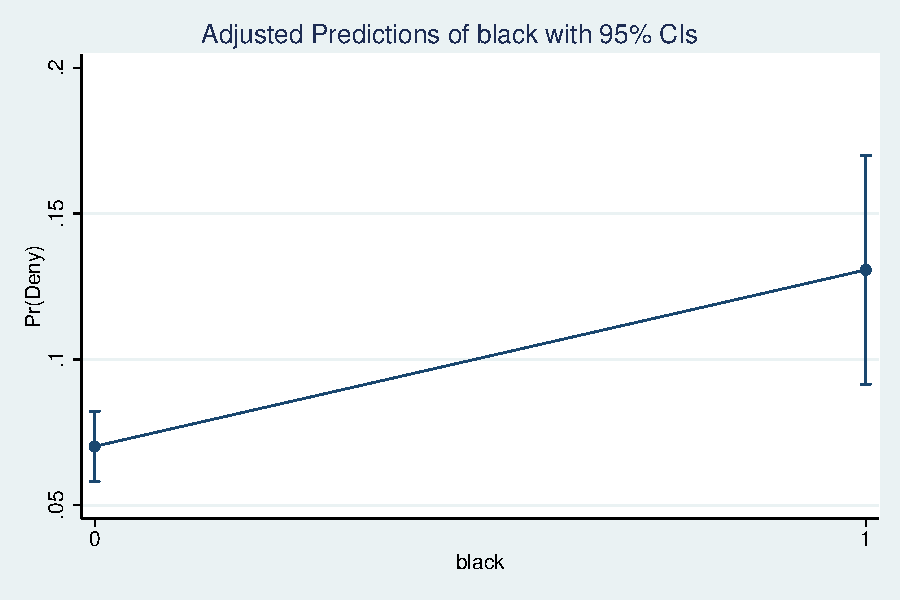
\includegraphics[]{stock_watson-11-Stata-fig.pdf}

%\begin{Statacode}
%\end{Statacode}

\end{document}
